\subsection{Convolutional Neural Network}

\begin{frame}
\frametitle{Biologische Zellarten}

\begin{figure}
	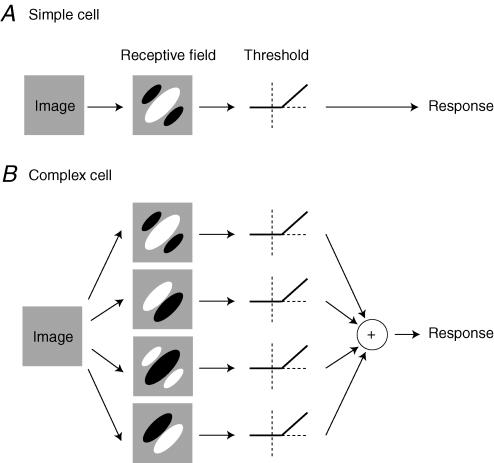
\includegraphics[width=.7\linewidth]{./aktuelleEntwicklung/convolutionalNN/img/simpleVsComplex_alpha}
\end{figure}


\note[item]{1962: zwei Neurophysiologen Torsten Wiesel und David Hubel}
\note[item]{Konzept der simple und complex cells}

\note[item]{nicht positionsbunden - spatial invariance, räumliche Invarianz}
\note[item]{Arten von Zellen zur Erkennung einfacher Kanten und Balken}
\note[item]{\emph{simple cells}: ist Positionsgebunden}
\note[item]{\emph{complex cells}: Muster können an beliebigen Positionen auftauchen}
\note[item]{1962: Konzept wie im Bild}
\note[item]{1980er Dr. Kunihiko Fukushima: erstes Modell nach diesem Konzept}

\end{frame}


\begin{frame}
\frametitle{Anfänge}

\begin{itemize}
\item Yann LeCun: erstes Modell zum Erkennen von Handschrift
\item \emph{Verwendung von MNIST database of handwritten digits}
\begin{itemize}
	\item 60.000 Trainingsdatensätze
	\item 10.000 zum Berechnen des Fehlers
\end{itemize}
\end{itemize}

\begin{figure}
	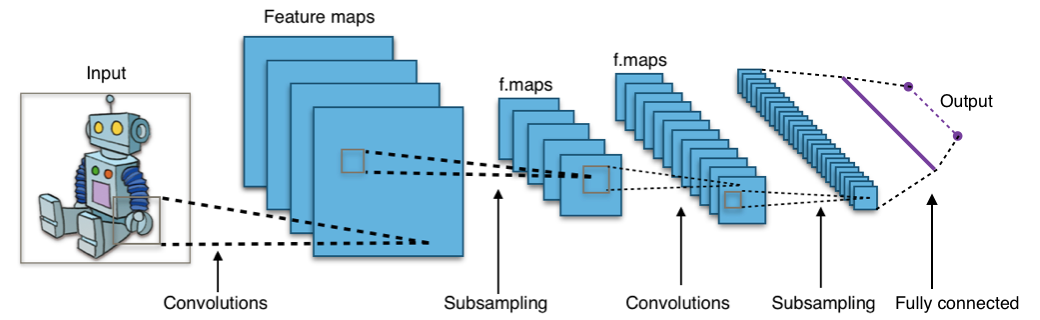
\includegraphics[width=.9\linewidth]{./aktuelleEntwicklung/convolutionalNN/img/cnn_overview_alpha}
\end{figure}


\note[item]{Pioniere, fr. Informatiker Yann LeCun}
\note[item]{Bekannteste Ausarbeitung über CNN für Handschriften}

\end{frame}


\begin{frame}
\frametitle{Convolutinal Layer - Filter}

\begin{itemize}
\item Mehrdimensionales Array mit Farbwerten zur Repräsentation im Rechner
\item Durch Filter auf bestimmte \emph{Low-Level} Eigenschaften schließen
\end{itemize}

\begin{figure}
	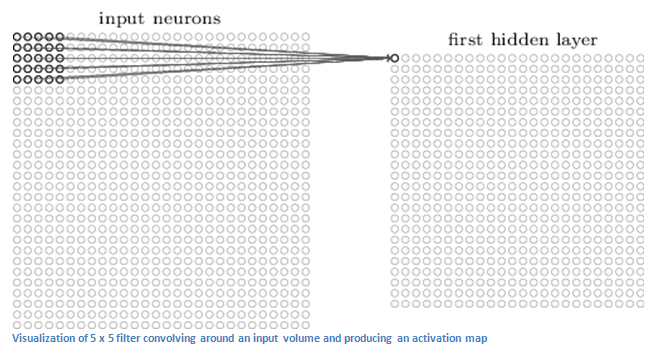
\includegraphics[width=.8\linewidth]{./aktuelleEntwicklung/convolutionalNN/img/cnn_convLayer_alpha}
\end{figure}

\note[item]{Farbwertearray kann pro Pixel mehrere Werte enthalten}
\end{frame}


\begin{frame}
\frametitle{Filter}


\begin{itemize}
\item Generell

\begin{itemize}
	\item Besitzt feste Pixelgröße (\emph{Kernelsize}) \& Schrittweite
	\item Scannt Bild Zeilenweise
	\item \emph{Padding} legt Verfahren für Rand des Bildes fest
	\item Ausgabe wird \emph{activation} oder \emph{feature map} genannt
\end{itemize}

\item Praxis
\begin{itemize}
	\item \emph{Convolutional Layer} mit 32 oder 16 Bit
	\item Jeder Filter generiert eigene Ausgabematrix
	\item Nächster Convolutional Layer verwendet Ausgabematrizen als Input
	\item Ausgabe wird in \emph{Pooling Layer} gesteckt
\end{itemize}

\end{itemize}


\note[item]{Bsp. Filter 2 x 2, Schrittweite: 2 - führt zu Halbierung der InputMatrix}
\note[item]{Im Bsp. hängen immer 4 Pixel an einem Filter, die Eingabematrix wird gefaltet (convolute)}

\end{frame}


\begin{frame}
\frametitle{Filter - Funktionsweise}

\begin{figure}
	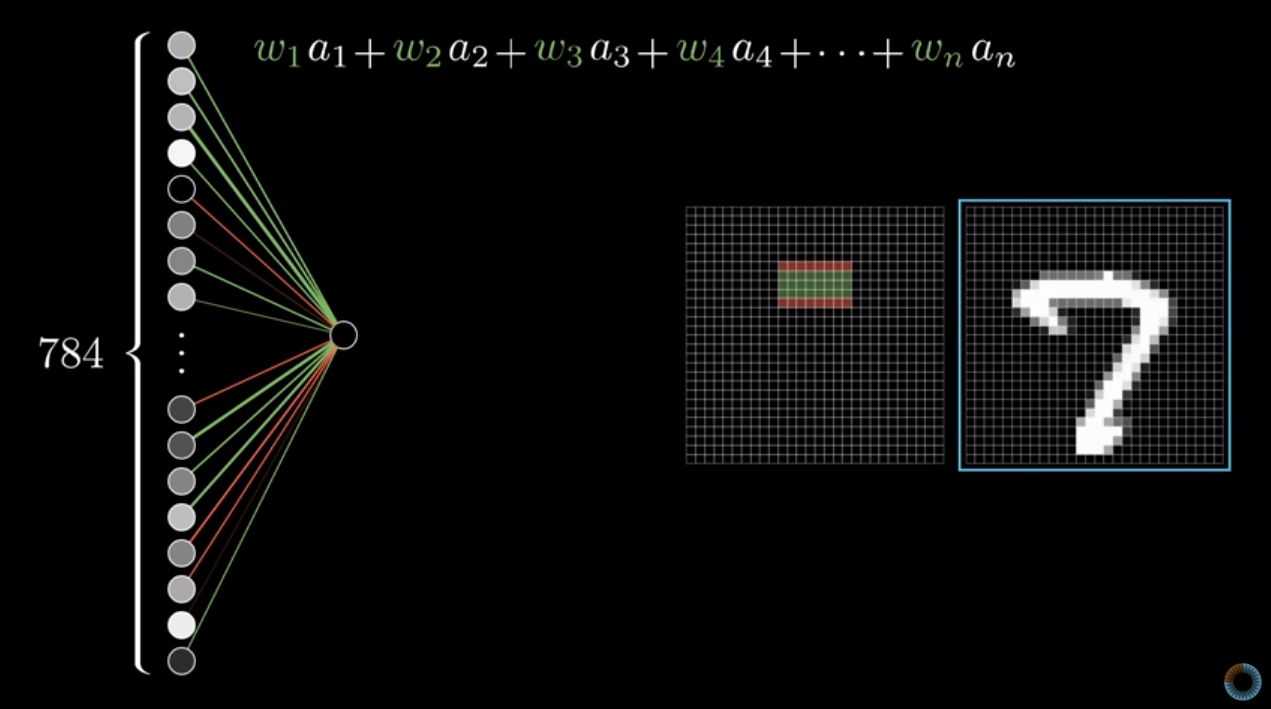
\includegraphics[width=\linewidth]{./aktuelleEntwicklung/convolutionalNN/img/filter}
\end{figure}
\end{frame}


\begin{frame}
\frametitle{Pooling Layer}

\begin{itemize}
\item Aggregiert die Ergebnisse von Convolutional Layern
\item Ziele
\begin{itemize}
	\item Nur die relevantesten Signale an nächste Schicht weitergeben
	\item Anzahl der Parameter im Netz reduzieren
\end{itemize}

\item \emph{MaxPooling Layer} am weitesten verbreitet
\end{itemize}


\note[item]{ während die Größe des Inputs durch die Faltungen und das Pooling immer weiter reduziert wird, erhöht sich die Anzahl der Filter zur Erkennung von übergeordneten Signalen zunehmend}

\end{frame}



\begin{frame}
\frametitle{Fully Connected Layer}

\begin{itemize}
\item Ausgagngspunkt: \emph{High-Level} Merkmale bereits durch frühere Schichten erkannt. 
\item Alle Neuronen der Ausgabeschicht sowie dieser Merkmale alle direkt miteinander verbunden
\item Ausgabe sollte mit den richtigen Gewichten / Schwellwerten relativ eindeutige Ausgaben generieren
\end{itemize}

\begin{figure}
	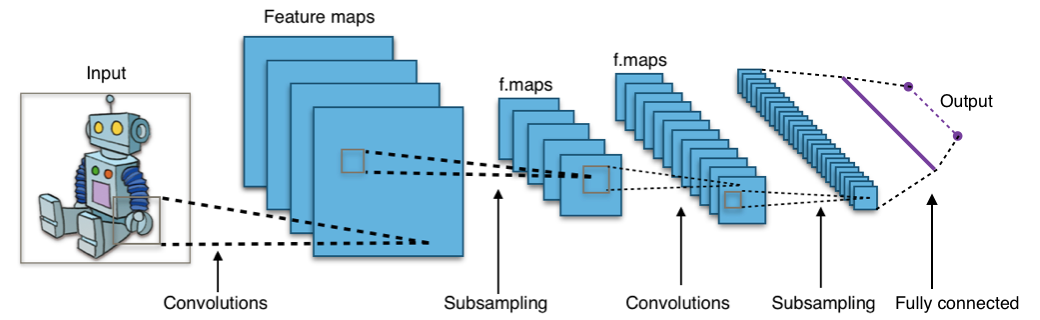
\includegraphics[width=.9\linewidth]{./aktuelleEntwicklung/convolutionalNN/img/cnn_overview_alpha}
\end{figure}


\end{frame}


